\documentclass[11pt,a4paper]{article}
\usepackage{float}
\usepackage{verbatim}
\usepackage{subfig}
\usepackage[T1]{fontenc}
\usepackage[utf8]{inputenc}
\usepackage{geometry}
\usepackage{enumitem}
%\geometry{verbose,lmargin=2cm,rmargin=2cm, bmargin=2cm, tmargin=2cm}
\usepackage{wrapfig}
\usepackage{tikz}
\usetikzlibrary{decorations.markings}
\usepackage{calc}
\usepackage{wrapfig}
\usepackage{graphicx}
\usepackage{amssymb}
\usepackage{amsmath}
\usepackage{esint}
\usepackage{multicol}
\usepackage{hyperref}
\usepackage{listings}
\hypersetup{
    colorlinks=true,
    linkcolor=blue,
    filecolor=magenta,
    urlcolor=cyan,
}
\usepackage{listings}
\lstset{ %
  backgroundcolor=\color{white},   % choose the background color; you must add \usepackage{color} or \usepackage{xcolor}; should come as last argument
  basicstyle=\footnotesize,        % the size of the fonts that are used for the code
  breakatwhitespace=false,         % sets if automatic breaks should only happen at whitespace
  breaklines=true,                 % sets automatic line breaking
  captionpos=t,                    % sets the caption-position to bottom
  commentstyle=\color{teal},    % comment style
  deletekeywords={...},            % if you want to delete keywords from the given language
  escapeinside={\%*}{*)},          % if you want to add LaTeX within your code
  extendedchars=true,              % lets you use non-ASCII characters; for 8-bits encodings only, does not work with UTF-8
  frame=single,                    % adds a frame around the code
  keepspaces=true,                 % keeps spaces in text, useful for keeping indentation of code (possibly needs columns=flexible)
  keywordstyle=\color{blue},       % keyword style
 % language=Python,                 % the language of the code
  morekeywords={*,...},           % if you want to add more keywords to the set
  numbers=left,                    % where to put the line-numbers; possible values are (none, left, right)
  numbersep=5pt,                   % how far the line-numbers are from the code
  numberstyle=\tiny\color{black}, % the style that is used for the line-numbers
  rulecolor=\color{black},         % if not set, the frame-color may be changed on line-breaks within not-black text (e.g. comments (green here))
  showspaces=false,                % show spaces everywhere adding particular underscores; it overrides 'showstringspaces'
  showstringspaces=false,          % underline spaces within strings only
  showtabs=false,                  % show tabs within strings adding particular underscores
  stepnumber=1,                    % the step between two line-numbers. If it's 1, each line will be numbered
  tabsize=2,                       % sets default tabsize to 2 spaces
  title=\lstname                   % show the filename of files included with \lstinputlisting; also try caption instead of title
}
\begin{document}



%\preprint{APS/123-QED}

\title{FYS2150 \\ Lab Report: Drag}% Force line breaks with \\

\author{Nicholas Karlsen}
% \email{nichoka@student.matnat.uio.no}

\date{\today}% It is always \today, today,
             %  but any date may be explicitly specified

\maketitle

\begin{abstract}
  A study on the flow of an assortment of spheres in a fluid and the use of image processing to determine the terminal velocity.
\end{abstract}

%\tableofcontents

\section{\label{sect:intro}Introduction}
  This report contains the description and analysis of data collected in the lab 21.03.2018 concerning the flow of several spherical objects in a large range of different sizes and densities. The balls were immersed in fluid, dropped and filmed. Post-lab, the raw footage was then processed using a Python script in order to quantify the motion of the spheres. This 

\section{\label{sect:theory}Theory}

  \subsection{Image processing\label{sect:imgpro}}

\section{\label{section:experimental}Experimental Procedure} 
  
  \subsection{Video capture\label{subsect:vidcap}}
    
    \begin{figure}[H]
      \center
      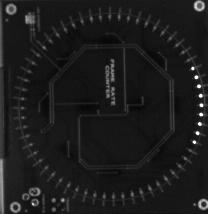
\includegraphics[width=7cm]{scripts/figs/sync_fps.png}
      \caption{Signal used to determine the FPS of the camera}
      \label{fig:FpsSignal}
    \end{figure}
  
    In order to capture the motion of the balls, a USB video camera was connected to a computer running uEye cockpit\cite{_ueye_????}, a program which allowed us to change the settings of the camera, as well as record video files. The image was set to grayscale and the contrast, exposure, gain etc was changed such that the color histogram in uEye would show two significant, separated peaks such that it would be easy to process the image using the method described in the theory section \ref{sect:imgpro}.

    Next, the error of the set FPS of the camera had to be determined. This was done by connecting a series of LEDs in a circle (see Fig. \ref{fig:FpsSignal}) to a signal generator. The light emitted would "circle" at a rate which could be changed using the signal generator. By adjusting the rate such that the emitted light would seem stationary when observed through the video feed in uEye, the true FPS of the camera could be determined. In our test, we set the camera to film at 60 FPS and the rate was adjusted untill the period of the LED was synced up with the camera at $3.60047$ KHz, the equivalent of $60.00783$ periods per second.

    In order to get the conversion factor between pixels and meters, a still picture was taken of the tubes with a known length in frame, at a distance roughly equal to where the balls would travel. This had to be done for each experimental setup. For our known lengths, we used a meter rule and a $30$ cm ruler for the large and small scale experiments respectively. See Fig. \ref{fig:scale1}.

    \begin{figure}[H]
      \center
      \subfloat[][Large tube]{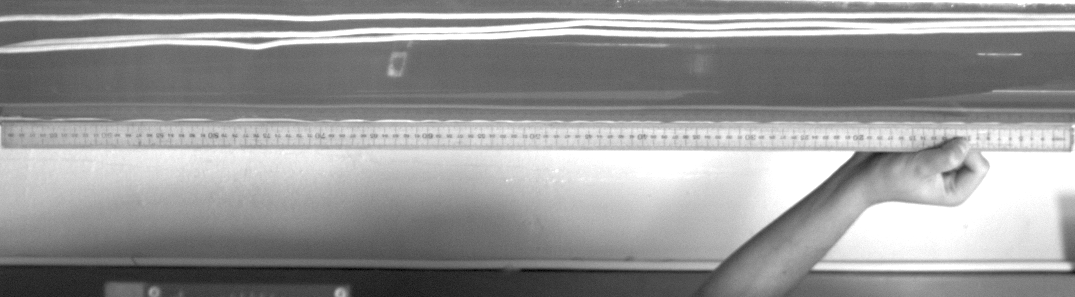
\includegraphics[width=8cm, angle=90]{scripts/figs/bilde_scale1.png}\label{<figure1>}}
      \subfloat[][Small tube]{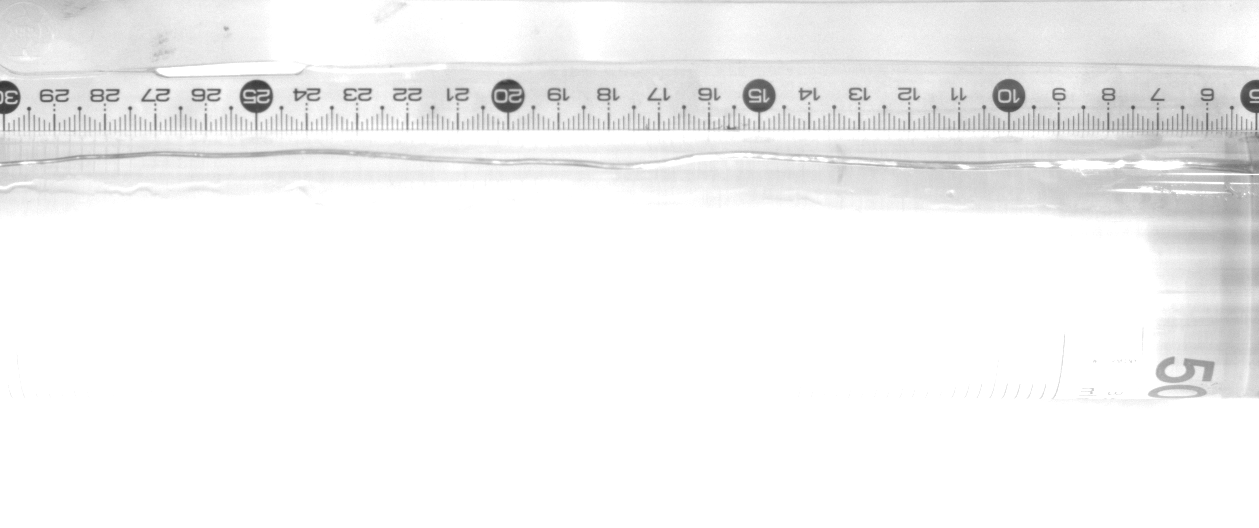
\includegraphics[width=8cm, angle=90]{scripts/figs/bilde_scale2.png}\label{<figure1>}}
      \caption{Cropped images used to find pixel to meter ratio for both of the tubes. (Scaled down in this document)}
      \label{fig:scale1}
    \end{figure}
  
  \subsection{Equipment}

    We had two similar experimental setups. One large scale, and one small scale. the large scale consisted of a roughly 2.5-3m tall\footnote{We did not measure the height of the tube, but it was fairly close to the ceiling.} transparrent tube, and the small scale a 30-40cm transparent measuring tube. Both of the tubes were filled with oil (Shell Tellus S2 M 68 Industrial Hydraulic Fluid\cite{_shell_????}).

    The set of balls which were to be dropped in the large scale setup are depicted in Fig. \ref{fig:balls}. Additionally, there were two smaller balls which were dropped in the small scale setup. The mass of the balls was measured using a digital scale with a precision of $0.01$g \cite{_proscale_????}, except for the two smallest balls, for which the mass was given by the lab instructor. The diameter of the balls was measured using a Vernier Caliper with a precision of $0.01$mm, again, except for the two smallest balls, which diameter was provided by the lab instructor.

    \begin{figure}[H]
      \center
      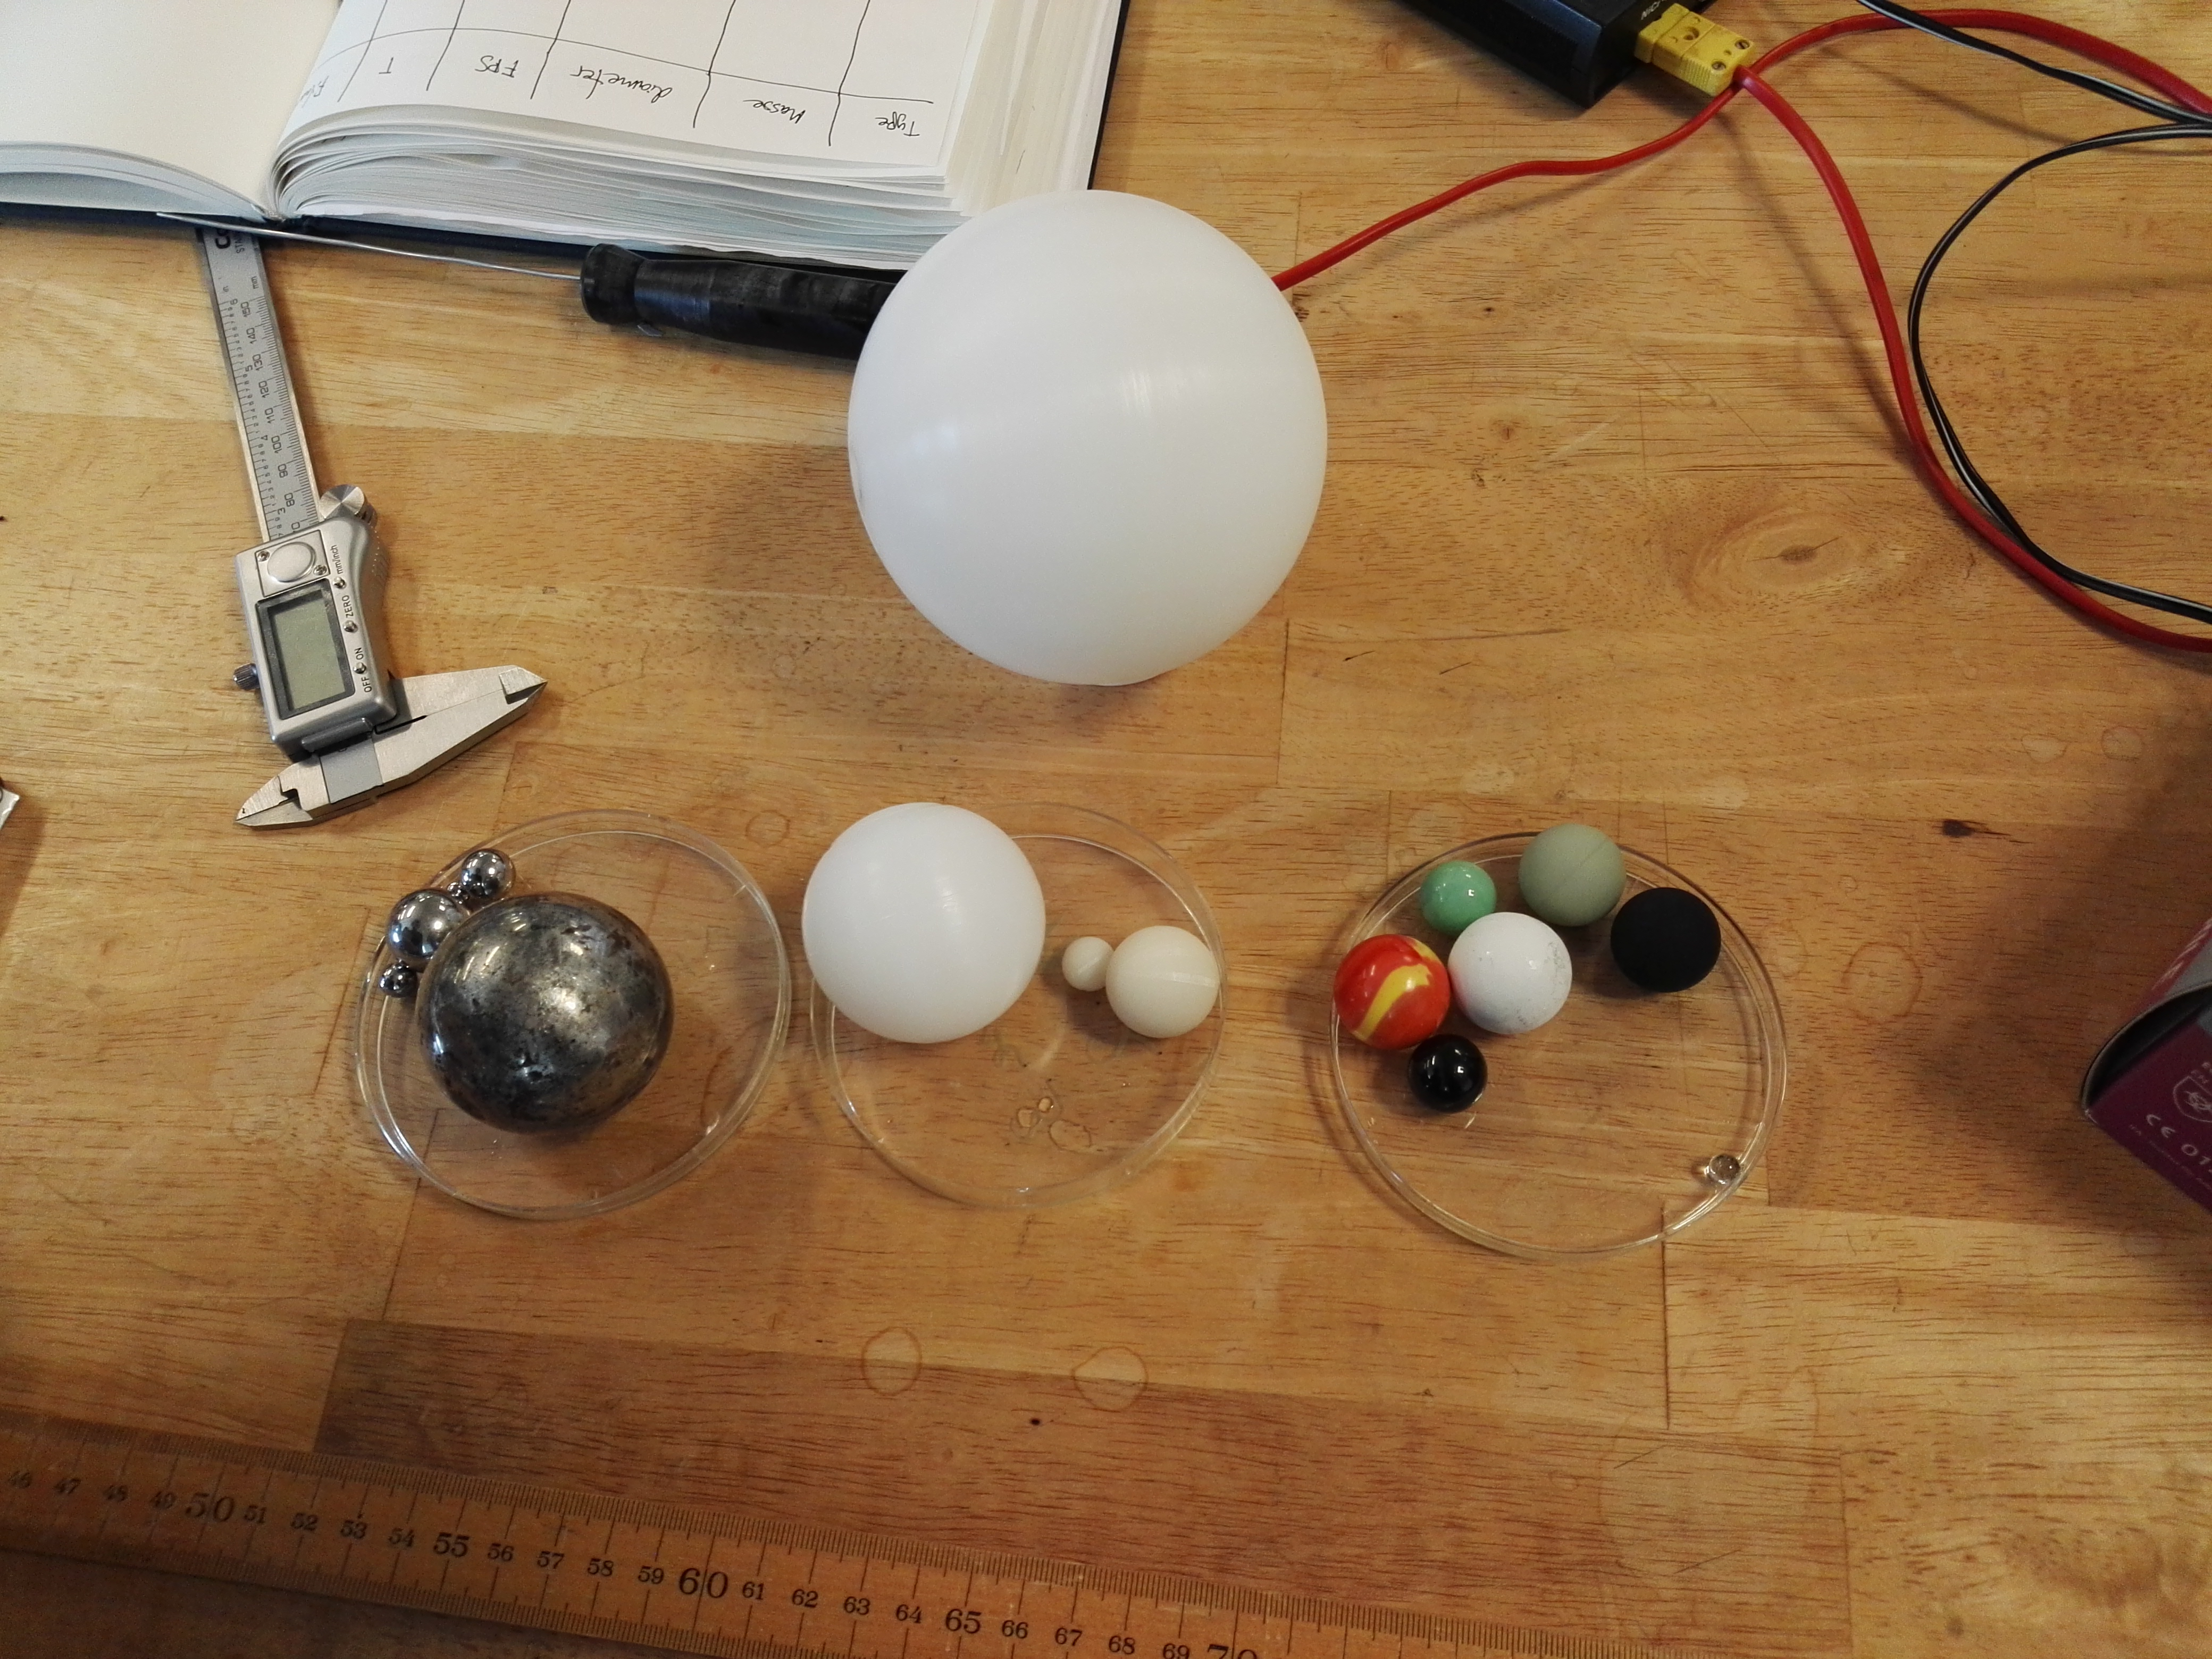
\includegraphics[width=7cm]{scripts/figs/IMG_20180321_131204.jpg}
      \caption{Most of the balls used in the experiment, excluding the ones labeled small 1 and 2.}
      \label{fig:balls}
    \end{figure}

  \subsection{Procedure}
    The experiment was performed by 3 people performing 3 different, simultaneous tasks. It can technically be performed by one person, but due to the nature of the experiment, it is not recommended, as it is not practical to make repeated readings if something goes wrong.

    The camera was pointed towards the large-scale tube, and prepared as described in section \ref{subsect:vidcap} between each reading. It was important that the lighting in the room was fairly constant for the video capture, so curtains were put in front of the windows. The camera was kept at 100 FPS for every experiment. For some of the balls with relatively low terminal velocity, the FPS could have been lowered to save space without making any significant sacrifices to the accuracy, but as we did not have any predicted values for the terminal velocity of the individual balls, we opted to keep it at 100FPS for every single experiment.

    Before each experiment, the temperature of the oil was measured using an IR-thermometer with a precision of $\pm2^\circ$C \cite{_fluke_????}. Which is used to determine the viscosity of the oil.

    For each experiment, a ball was picked up by hand and brought to the top of the tube by ladder. The ball was gripped tightly before carefully submerging it in the oil. After having ensured the person operating the camera software was ready to record, the ball was dropped. It was critical that the ball was dropped in a certain way, otherwise it gained too much horizontal velocity, which at worst could cause it to hit the side of the tube halfway through\footnote{Which happened in our first attempt} the tube. In order to avoid this, it is important to separate the fingers gripping the ball at the same time when dropping it, instead of letting it slide out of the hand. Sliding it out, leads it to spin, which in turn may lead it to move horizontally.

    The same procedure was performed for the small-scale experiments.
    



\section{\label{sect:results}Results}

  \begin{table}[H]
    \center
    \caption{Results}
    \begin{tabular}{ r | l  l l  r  r  r }
      \input{scripts/data/labdata.dat} 
    \end{tabular}
    \label{tab:results}
  \end{table}


\section{\label{sect:discuss}Discussion}
\section{\label{sect:conclusion}Conclusion}

\bibliographystyle{plain}
\bibliography{references.bib} 



%%%%%%%%%%%%%%%%%%%%%%%%
%%% END OF MAIN BODY %%%
%%%%%%%%%%%%%%%%%%%%%%%%

%\appendix*
%\section{Scripts}
%\lstinputlisting[language=python]{scripts/lesVideo_conv.py}
%\lstinputlisting{scripts/data/labdata.dat}

\end{document}